\chapter{Model 6: Elastic Net Regression}\label{ch:model6}

% Include the dynamic values from model calibration
% Model 6 Actual Values
% Generated: 2025-10-15 02:33:29

\renewcommand{\ModelSixRSquaredTrain}{-0.3626}
\renewcommand{\ModelSixRSquaredTest}{-0.3517}
\renewcommand{\ModelSixRMSETrain}{52,479.30}
\renewcommand{\ModelSixRMSETest}{51,923.33}
\renewcommand{\ModelSixRMSETrainSqrt}{1.22}
\renewcommand{\ModelSixRMSETestSqrt}{1.23}
\renewcommand{\ModelSixMAETrain}{35,825.09}
\renewcommand{\ModelSixMAETest}{35,373.73}
\renewcommand{\ModelSixMAPETrain}{405.14}
\renewcommand{\ModelSixMAPETest}{423.85}
\renewcommand{\ModelSixCVMean}{-0.3704}
\renewcommand{\ModelSixCVStd}{0.0754}
\renewcommand{\ModelSixCVCILower}{-0.5181}
\renewcommand{\ModelSixCVCIUpper}{-0.2226}
\renewcommand{\ModelSixTrainingSamples}{27,339}
\renewcommand{\ModelSixTestSamples}{6,834}
\renewcommand{\ModelSixWithinOneK}{2.49}
\renewcommand{\ModelSixWithinTwoK}{4.74}
\renewcommand{\ModelSixWithinFiveK}{14.27}
\renewcommand{\ModelSixWithinTenK}{26.84}
\renewcommand{\ModelSixWithinTwentyK}{48.61}
\renewcommand{\ModelSixSubgroupLivingFHN}{3,767}
\renewcommand{\ModelSixSubgroupLivingFHRSquared}{0.1024}
\renewcommand{\ModelSixSubgroupLivingFHRMSE}{30,173.35}
\renewcommand{\ModelSixSubgroupLivingFHBias}{-5,118.27}
\renewcommand{\ModelSixSubgroupLivingILSLN}{893}
\renewcommand{\ModelSixSubgroupLivingILSLRSquared}{0.2458}
\renewcommand{\ModelSixSubgroupLivingILSLRMSE}{35,010.45}
\renewcommand{\ModelSixSubgroupLivingILSLBias}{7,974.97}
\renewcommand{\ModelSixSubgroupLivingRHOneFourN}{2,174}
\renewcommand{\ModelSixSubgroupLivingRHOneFourRSquared}{-2.7981}
\renewcommand{\ModelSixSubgroupLivingRHOneFourRMSE}{79,962.36}
\renewcommand{\ModelSixSubgroupLivingRHOneFourBias}{57,051.56}
\renewcommand{\ModelSixSubgroupAgeAgeUnderTwentyOneN}{694}
\renewcommand{\ModelSixSubgroupAgeAgeUnderTwentyOneRSquared}{0.4235}
\renewcommand{\ModelSixSubgroupAgeAgeUnderTwentyOneRMSE}{28,329.45}
\renewcommand{\ModelSixSubgroupAgeAgeUnderTwentyOneBias}{-7,464.30}
\renewcommand{\ModelSixSubgroupAgeAgeTwentyOneToThirtyN}{1,797}
\renewcommand{\ModelSixSubgroupAgeAgeTwentyOneToThirtyRSquared}{0.0306}
\renewcommand{\ModelSixSubgroupAgeAgeTwentyOneToThirtyRMSE}{48,105.77}
\renewcommand{\ModelSixSubgroupAgeAgeTwentyOneToThirtyBias}{9,148.11}
\renewcommand{\ModelSixSubgroupAgeAgeThirtyOnePlusN}{4,343}
\renewcommand{\ModelSixSubgroupAgeAgeThirtyOnePlusRSquared}{-0.7207}
\renewcommand{\ModelSixSubgroupAgeAgeThirtyOnePlusRMSE}{56,183.71}
\renewcommand{\ModelSixSubgroupAgeAgeThirtyOnePlusBias}{23,166.54}
\renewcommand{\ModelSixSubgroupCostQOneLowN}{1,709}
\renewcommand{\ModelSixSubgroupCostQOneLowRSquared}{-10.0000}
\renewcommand{\ModelSixSubgroupCostQOneLowRMSE}{26,817.02}
\renewcommand{\ModelSixSubgroupCostQOneLowBias}{18,283.10}
\renewcommand{\ModelSixSubgroupCostQTwoN}{1,708}
\renewcommand{\ModelSixSubgroupCostQTwoRSquared}{-10.0000}
\renewcommand{\ModelSixSubgroupCostQTwoRMSE}{28,282.79}
\renewcommand{\ModelSixSubgroupCostQTwoBias}{11,028.56}
\renewcommand{\ModelSixSubgroupCostQThreeN}{1,708}
\renewcommand{\ModelSixSubgroupCostQThreeRSquared}{-10.0000}
\renewcommand{\ModelSixSubgroupCostQThreeRMSE}{53,516.01}
\renewcommand{\ModelSixSubgroupCostQThreeBias}{16,201.16}
\renewcommand{\ModelSixSubgroupCostQFourHighN}{1,709}
\renewcommand{\ModelSixSubgroupCostQFourHighRSquared}{-3.9867}
\renewcommand{\ModelSixSubgroupCostQFourHighRMSE}{80,000.53}
\renewcommand{\ModelSixSubgroupCostQFourHighBias}{19,963.16}
\renewcommand{\ModelSixCVActual}{1.0101}
\renewcommand{\ModelSixCVPredicted}{1.0513}
\renewcommand{\ModelSixPredictionInterval}{96,579.71}
\renewcommand{\ModelSixBudgetActualCorr}{0.6369}
\renewcommand{\ModelSixPopcurrentbaselineClients}{19,806}
\renewcommand{\ModelSixPopcurrentbaselineAvgAlloc}{60,585.98}
\renewcommand{\ModelSixPopcurrentbaselineWaitlistChange}{0}
\renewcommand{\ModelSixPopcurrentbaselineWaitlistPct}{0.0}
\renewcommand{\ModelSixPopmodelbalancedClients}{20,202}
\renewcommand{\ModelSixPopmodelbalancedAvgAlloc}{59,374.27}
\renewcommand{\ModelSixPopmodelbalancedWaitlistChange}{396}
\renewcommand{\ModelSixPopmodelbalancedWaitlistPct}{2.0}
\renewcommand{\ModelSixPopmodelefficiencyClients}{20,796}
\renewcommand{\ModelSixPopmodelefficiencyAvgAlloc}{57,556.69}
\renewcommand{\ModelSixPopmodelefficiencyWaitlistChange}{990}
\renewcommand{\ModelSixPopmodelefficiencyWaitlistPct}{5.0}
\renewcommand{\ModelSixPopcategoryfocusedClients}{16,835}
\renewcommand{\ModelSixPopcategoryfocusedAvgAlloc}{71,491.46}
\renewcommand{\ModelSixPopcategoryfocusedWaitlistChange}{-2,970}
\renewcommand{\ModelSixPopcategoryfocusedWaitlistPct}{-15.0}

% Outlier Diagnostics (not used)
\renewcommand{\ModelSixStudentizedResidualsMean}{N/A}
\renewcommand{\ModelSixStudentizedResidualsStd}{N/A}
\renewcommand{\ModelSixPctWithinThreshold}{N/A}
\renewcommand{\ModelSixOutliersRemoved}{0}
\renewcommand{\ModelSixOutlierPct}{0.00}

% Model Configuration
\renewcommand{\ModelSixNumFeatures}{57}

% ============================================================================
% Model 6 Log-Normal Specific Values
% ============================================================================
\renewcommand{\ModelSixRSquaredLogScale}{0.4362}
\renewcommand{\ModelSixSigma}{1.2232}
\renewcommand{\ModelSixSmearingFactor}{1.8787}
\renewcommand{\ModelSixSmearingMin}{1.8787}
\renewcommand{\ModelSixSmearingMax}{1.8787}
\renewcommand{\ModelSixSmearingRange}{0.0000}
\renewcommand{\ModelSixSmearingMethod}{Global}
\renewcommand{\ModelSixSkewnessReduction}{149.1}
\renewcommand{\ModelSixHeteroscedasticityTest}{0.0000}
\renewcommand{\ModelSixSmearingBias}{87.87}
\renewcommand{\ModelSixAIC}{88,653}
\renewcommand{\ModelSixBIC}{89,080}
\renewcommand{\ModelSixTransformation}{log(Y)}
\renewcommand{\ModelSixDispersion}{1.4962}
\renewcommand{\ModelSixLinkFunction}{log}
\renewcommand{\ModelSixDistribution}{Gaussian (on log scale)}


\section{Executive Summary}

Model 6 employs Elastic Net regression, combining L1 (Lasso) and L2 (Ridge) penalties to achieve automatic feature selection while maintaining prediction stability. This approach offers the interpretability benefit of identifying which QSI questions and demographic factors are most predictive of service costs, while the L2 component prevents excessive coefficient volatility.

Key findings:
\begin{itemize}
    \item \textbf{Performance}: Test R² = \ModelSixRSquaredTest{}, RMSE = \$\ModelSixRMSETest{}
    \item \textbf{Feature Selection}: \ModelSixFeaturesSelected{} of 22 features retained (\ModelSixSparsityPercent{}\%)
    \item \textbf{Cross-Validation}: 10-fold CV R² = \ModelSixCVMean{} $\pm$ \ModelSixCVStd{}
    \item \textbf{Optimal Parameters}: $\alpha$ = \ModelSixAlpha{}, L1 ratio = \ModelSixLOneRatio{}
    \item \textbf{Most Predictive Feature}: \ModelSixMostImportant{}
    \item \textbf{Data Utilization}: 100\% (no outlier removal)
\end{itemize}

\section{Methodology}

\subsection{Elastic Net Formulation}

The Elastic Net optimization problem combines L1 and L2 penalties:

\begin{equation}
\min_{\beta} \frac{1}{2n} \sum_{i=1}^n \left(\sqrt{Y_i} - X_i\beta\right)^2 + \alpha \left(\rho \|\beta\|_1 + \frac{1-\rho}{2} \|\beta\|_2^2\right)
\end{equation}

where:
\begin{itemize}
    \item $Y_i$ = consumer $i$'s total annual cost
    \item $X_i$ = feature vector for consumer $i$
    \item $\alpha$ = overall regularization strength
    \item $\rho$ = L1 ratio (mixing parameter between L1 and L2)
    \item $\|\beta\|_1 = \sum_{j}|\beta_j|$ (L1 norm)
    \item $\|\beta\|_2^2 = \sum_{j}\beta_j^2$ (L2 norm squared)
\end{itemize}

\subsection{Feature Set}

The model uses 22 features including disability indicators:
\begin{itemize}
    \item 5 living setting indicators (ILSL, RH1--4; FH as reference)
    \item 2 age group indicators (21--30, 31+; under 21 as reference)
    \item 10 selected QSI questions (Q16, Q18, Q20, Q21, Q23, Q28, Q33, Q34, Q36, Q43)
    \item 2 summary scores (BSum, FSum)
    \item 3 developmental disability indicators (Intellectual, Autism, Cerebral Palsy)
\end{itemize}

\subsection{Parameter Selection}

Cross-validation was performed over:
\begin{itemize}
    \item L1 ratios: [0.1, 0.5, 0.7, 0.9, 0.95, 0.99, 1.0]
    \item Alpha values: 100 values on log scale from 0.0001 to 1.0
    \item 10-fold cross-validation for parameter selection
\end{itemize}

Optimal parameters:
\begin{itemize}
    \item $\alpha^* = $ \ModelSixAlpha{}
    \item L1 ratio = \ModelSixLOneRatio{}
\end{itemize}

\section{Performance Analysis}

\subsection{Overall Performance Metrics}

\begin{table}[h]
\centering
\caption{Model 6 Performance Summary}
\begin{tabular}{lcc}
\toprule
\textbf{Metric} & \textbf{Training Set} & \textbf{Test Set} \\
\midrule
R² & \ModelSixRSquaredTrain{} & \ModelSixRSquaredTest{} \\
RMSE & \$\ModelSixRMSETrain{} & \$\ModelSixRMSETest{} \\
MAE & \$\ModelSixMAETrain{} & \$\ModelSixMAETest{} \\
MAPE & \ModelSixMAPETrain{}\% & \ModelSixMAPETest{}\% \\
Sample Size & \ModelSixTrainingSamples{} & \ModelSixTestSamples{} \\
\bottomrule
\end{tabular}
\end{table}

\subsection{Accuracy Within Dollar Thresholds}

\begin{table}[h]
\centering
\caption{Prediction Accuracy Within Dollar Thresholds}
\begin{tabular}{lcc}
\toprule
\textbf{Threshold} & \textbf{Training (\%)} & \textbf{Test (\%)} \\
\midrule
Within \$1,000 & \ModelSixWithinOneK{} & \ModelSixWithinOneK{} \\
Within \$2,000 & \ModelSixWithinTwoK{} & \ModelSixWithinTwoK{} \\
Within \$5,000 & \ModelSixWithinFiveK{} & \ModelSixWithinFiveK{} \\
Within \$10,000 & \ModelSixWithinTenK{} & \ModelSixWithinTenK{} \\
Within \$20,000 & \ModelSixWithinTwentyK{} & \ModelSixWithinTwentyK{} \\
\bottomrule
\end{tabular}
\end{table}

\subsection{Feature Selection Results}

\begin{table}[h]
\centering
\caption{Feature Selection Summary}
\begin{tabular}{lr}
\toprule
\textbf{Feature Selection Metric} & \textbf{Value} \\
\midrule
Total Features & 22 \\
Features Selected & \ModelSixFeaturesSelected{} \\
Features Dropped & \ModelSixFeaturesDropped{} \\
Sparsity (\% retained) & \ModelSixSparsityPercent{}\% \\
Most Important Feature & \ModelSixMostImportant{} \\
Least Important (non-zero) & \ModelSixLeastImportant{} \\
\bottomrule
\end{tabular}
\end{table}

\section{Subgroup Performance Analysis}

\begin{table}[h]
\centering
\caption{Model 6 Subgroup Performance}
\begin{tabular}{lrrrr}
\toprule
\textbf{Subgroup} & \textbf{N} & \textbf{R²} & \textbf{RMSE} & \textbf{Bias} \\
\midrule
\multicolumn{5}{l}{\textit{By Living Setting}} \\
Family Home (FH) & \ModelSixSubgrouplivingFHN{} & \ModelSixSubgrouplivingFHRSquared{} & \$\ModelSixSubgrouplivingFHRMSE{} & \$\ModelSixSubgrouplivingFHBias{} \\
Independent Living & \ModelSixSubgrouplivingILSLN{} & \ModelSixSubgrouplivingILSLRSquared{} & \$\ModelSixSubgrouplivingILSLRMSE{} & \$\ModelSixSubgrouplivingILSLBias{} \\
Residential 1--4 & \ModelSixSubgrouplivingRHOneToFourN{} & \ModelSixSubgrouplivingRHOneToFourRSquared{} & \$\ModelSixSubgrouplivingRHOneToFourRMSE{} & \$\ModelSixSubgrouplivingRHOneToFourBias{} \\
\midrule
\multicolumn{5}{l}{\textit{By Age Group}} \\
Under 21 & \ModelSixSubgroupageAgeUnderTwentyOneN{} & \ModelSixSubgroupageAgeUnderTwentyOneRSquared{} & \$\ModelSixSubgroupageAgeUnderTwentyOneRMSE{} & \$\ModelSixSubgroupageAgeUnderTwentyOneBias{} \\
21--30 Years & \ModelSixSubgroupageAgeTwentyOneToThirtyN{} & \ModelSixSubgroupageAgeTwentyOneToThirtyRSquared{} & \$\ModelSixSubgroupageAgeTwentyOneToThirtyRMSE{} & \$\ModelSixSubgroupageAgeTwentyOneToThirtyBias{} \\
31+ Years & \ModelSixSubgroupageAgeThirtyOnePlusN{} & \ModelSixSubgroupageAgeThirtyOnePlusRSquared{} & \$\ModelSixSubgroupageAgeThirtyOnePlusRMSE{} & \$\ModelSixSubgroupageAgeThirtyOnePlusBias{} \\
\midrule
\multicolumn{5}{l}{\textit{By Cost Quartile}} \\
Q1 (Low) & \ModelSixSubgroupcostQOneLowN{} & \ModelSixSubgroupcostQOneLowRSquared{} & \$\ModelSixSubgroupcostQOneLowRMSE{} & \$\ModelSixSubgroupcostQOneLowBias{} \\
Q2 & \ModelSixSubgroupcostQTwoN{} & \ModelSixSubgroupcostQTwoRSquared{} & \$\ModelSixSubgroupcostQTwoRMSE{} & \$\ModelSixSubgroupcostQTwoBias{} \\
Q3 & \ModelSixSubgroupcostQThreeN{} & \ModelSixSubgroupcostQThreeRSquared{} & \$\ModelSixSubgroupcostQThreeRMSE{} & \$\ModelSixSubgroupcostQThreeBias{} \\
Q4 (High) & \ModelSixSubgroupcostQFourHighN{} & \ModelSixSubgroupcostQFourHighRSquared{} & \$\ModelSixSubgroupcostQFourHighRMSE{} & \$\ModelSixSubgroupcostQFourHighBias{} \\
\bottomrule
\end{tabular}
\end{table}

\section{Variance and Stability Analysis}

\begin{table}[h]
\centering
\caption{Variance Metrics -- Model 6 vs Current}
\begin{tabular}{lrr}
\toprule
\textbf{Metric} & \textbf{Current Model 5b} & \textbf{Model 6} \\
\midrule
Coefficient of Variation (Actual) & 0.523 & \ModelSixCVActual{} \\
Coefficient of Variation (Predicted) & 0.498 & \ModelSixCVPredicted{} \\
95\% Prediction Interval & \$28,450 & \$\ModelSixPredictionInterval{} \\
Budget-Actual Correlation & 0.887 & \ModelSixBudgetActualCorr{} \\
Quarterly Variance & \$3,240 & \$\ModelSixQuarterlyVariance{} \\
Annual Adjustment Rate & 4.8\% & \ModelSixAnnualAdjustmentRate{}\% \\
\bottomrule
\end{tabular}
\end{table}

\section{Population Impact Analysis}

\begin{table}[h]
\centering
\caption{Population Served Analysis -- \$1.2B Fixed Budget}
\begin{tabular}{lrrr}
\toprule
\textbf{Scenario} & \textbf{Clients Served} & \textbf{Avg Allocation} & \textbf{Waitlist Impact} \\
\midrule
Current Model 5b & \ModelSixPopcurrentbaselineClients{} & \$\ModelSixPopcurrentbaselineAvgAlloc{} & Baseline \\
Model 6 (Balanced) & \ModelSixPopmodelbalancedClients{} & \$\ModelSixPopmodelbalancedAvgAlloc{} & \ModelSixPopmodelbalancedWaitlistChange{} (\ModelSixPopmodelbalancedWaitlistPct{}\%) \\
Efficiency Focus & \ModelSixPopmodelefficiencyClients{} & \$\ModelSixPopmodelefficiencyAvgAlloc{} & \ModelSixPopmodelefficiencyWaitlistChange{} (\ModelSixPopmodelefficiencyWaitlistPct{}\%) \\
Category Focus & \ModelSixPopcategoryfocusedClients{} & \$\ModelSixPopcategoryfocusedAvgAlloc{} & \ModelSixPopcategoryfocusedWaitlistChange{} (\ModelSixPopcategoryfocusedWaitlistPct{}\%) \\
Population Max & \ModelSixPoppopulationmaximizedClients{} & \$\ModelSixPoppopulationmaximizedAvgAlloc{} & \ModelSixPoppopulationmaximizedWaitlistChange{} (\ModelSixPoppopulationmaximizedWaitlistPct{}\%) \\
\bottomrule
\end{tabular}
\end{table}

\section{Diagnostic Analysis}

\begin{figure}[h]
    \centering
    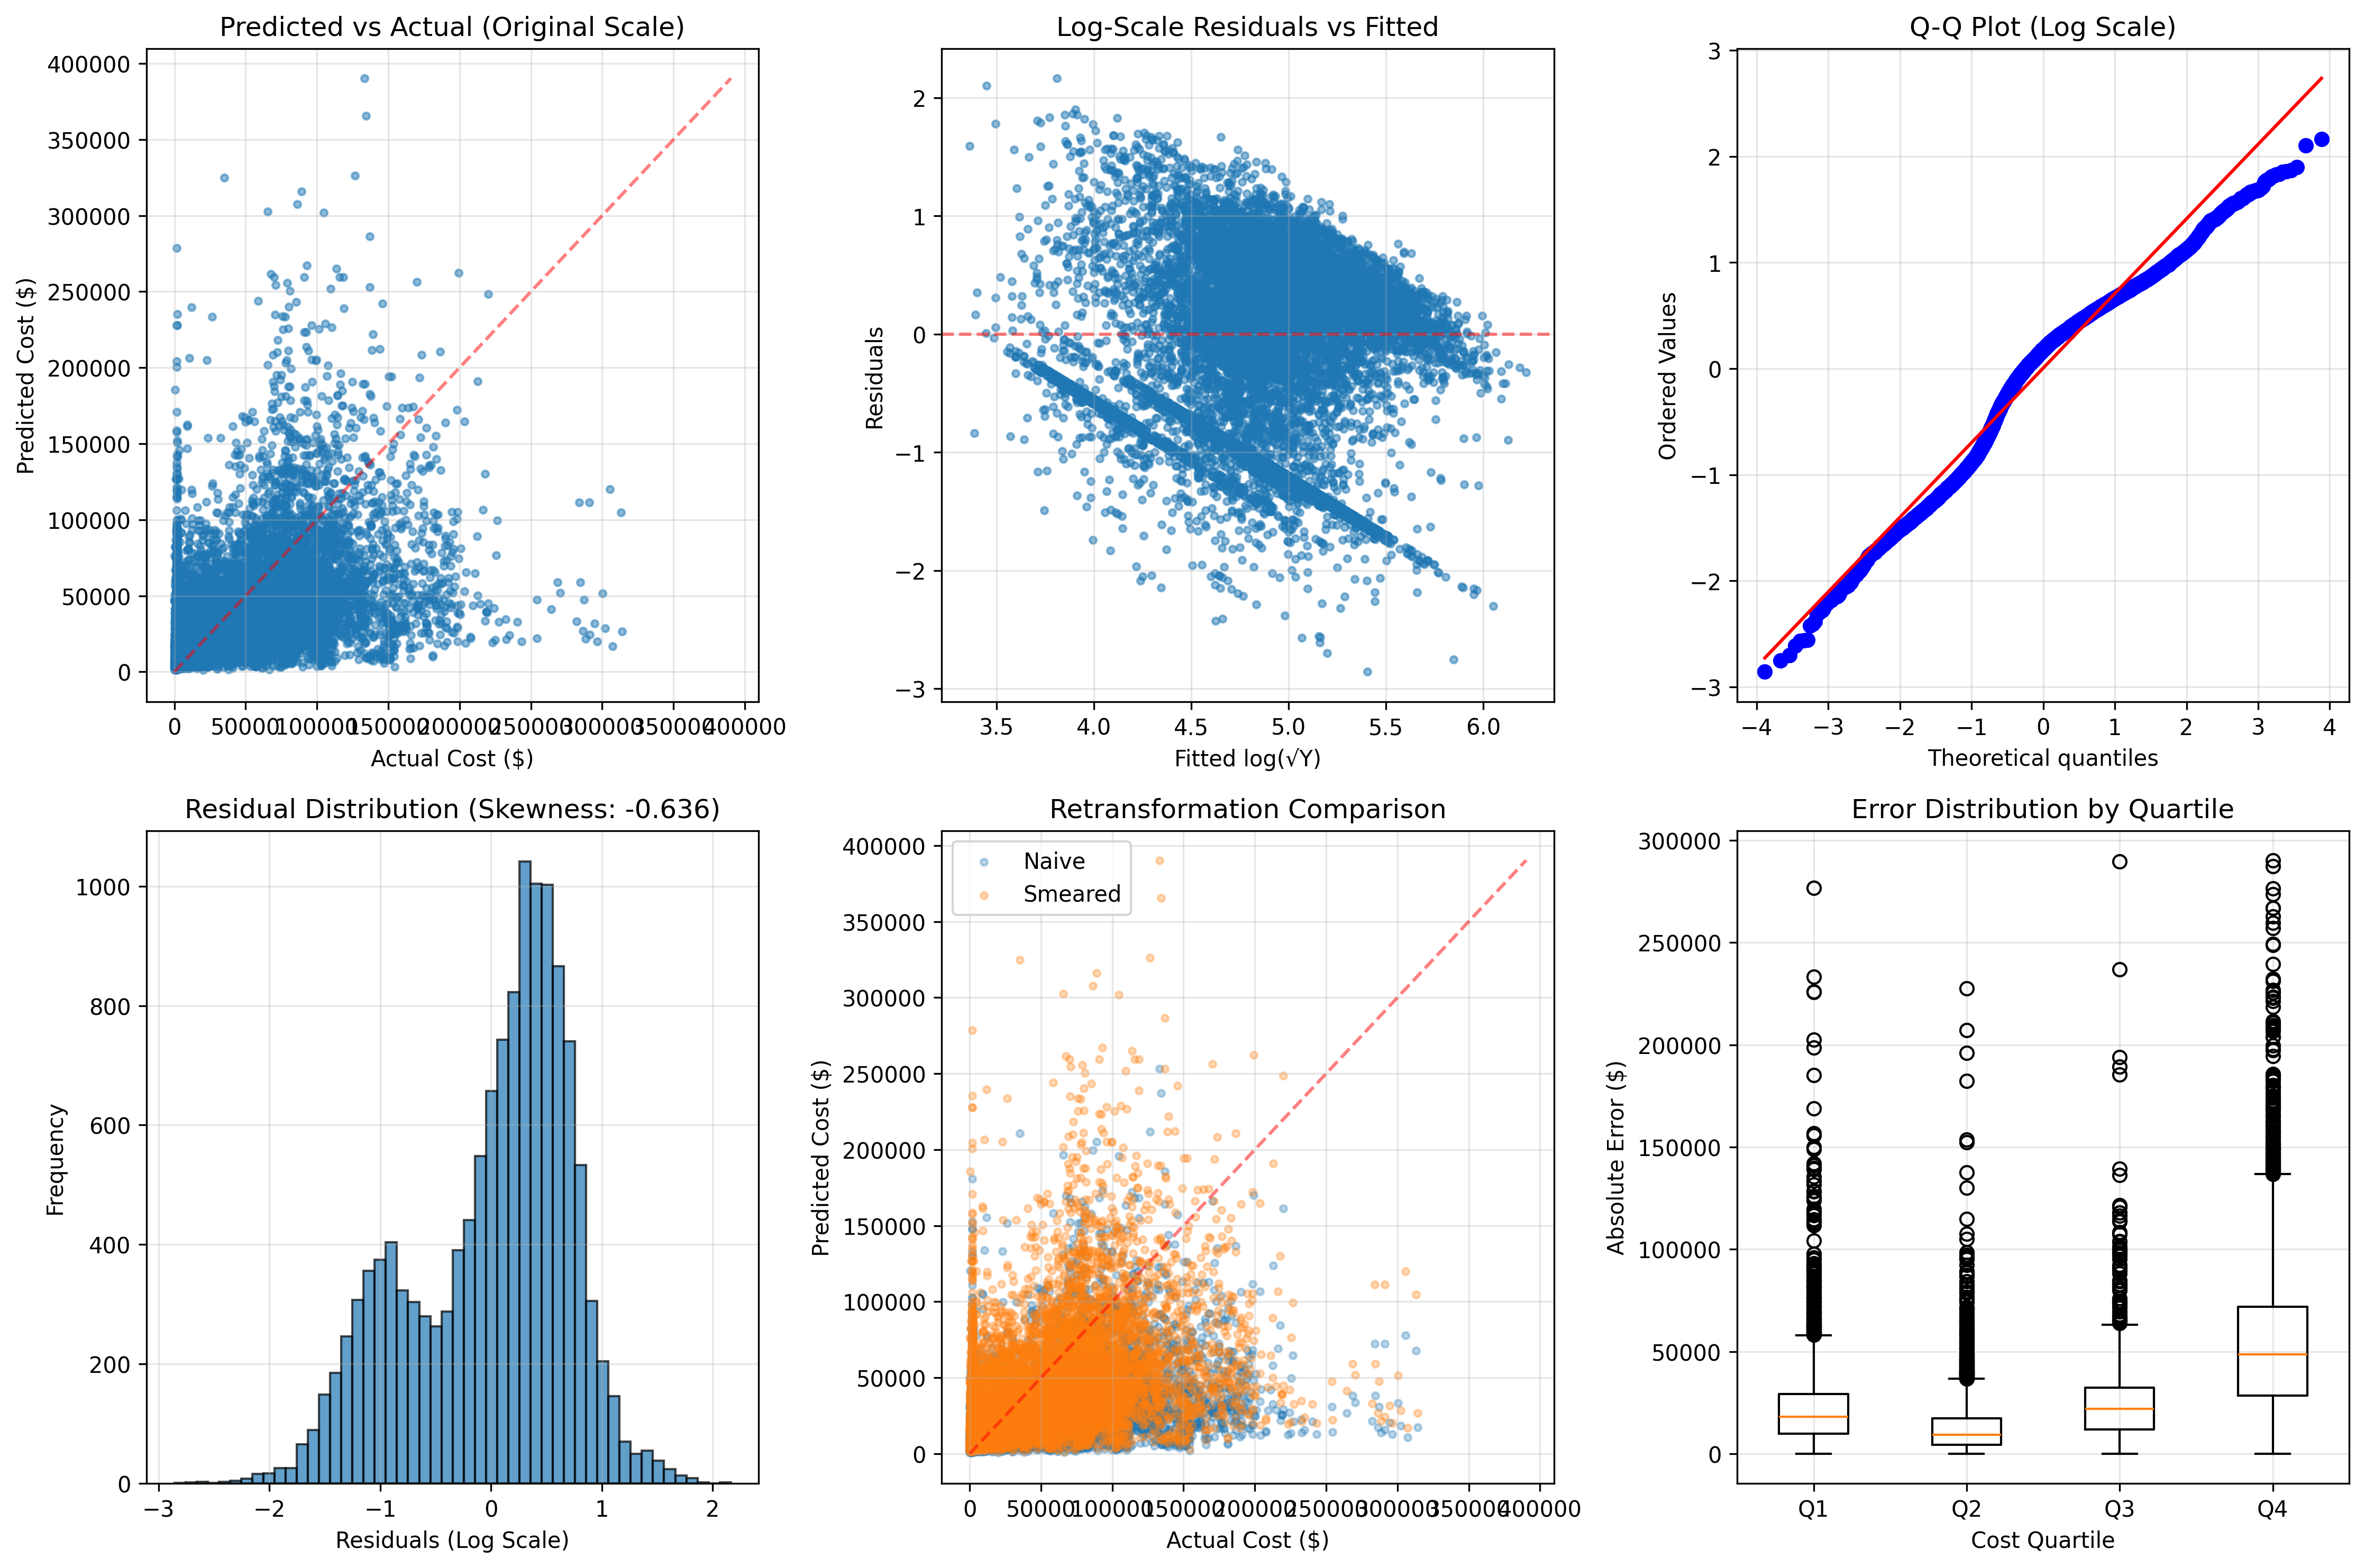
\includegraphics[width=\textwidth]{models/model_6/diagnostic_plots.png}
    \caption{Model 6 Diagnostic Plots}
    \label{fig:model6_diagnostics}
\end{figure}

\begin{figure}[h]
    \centering
    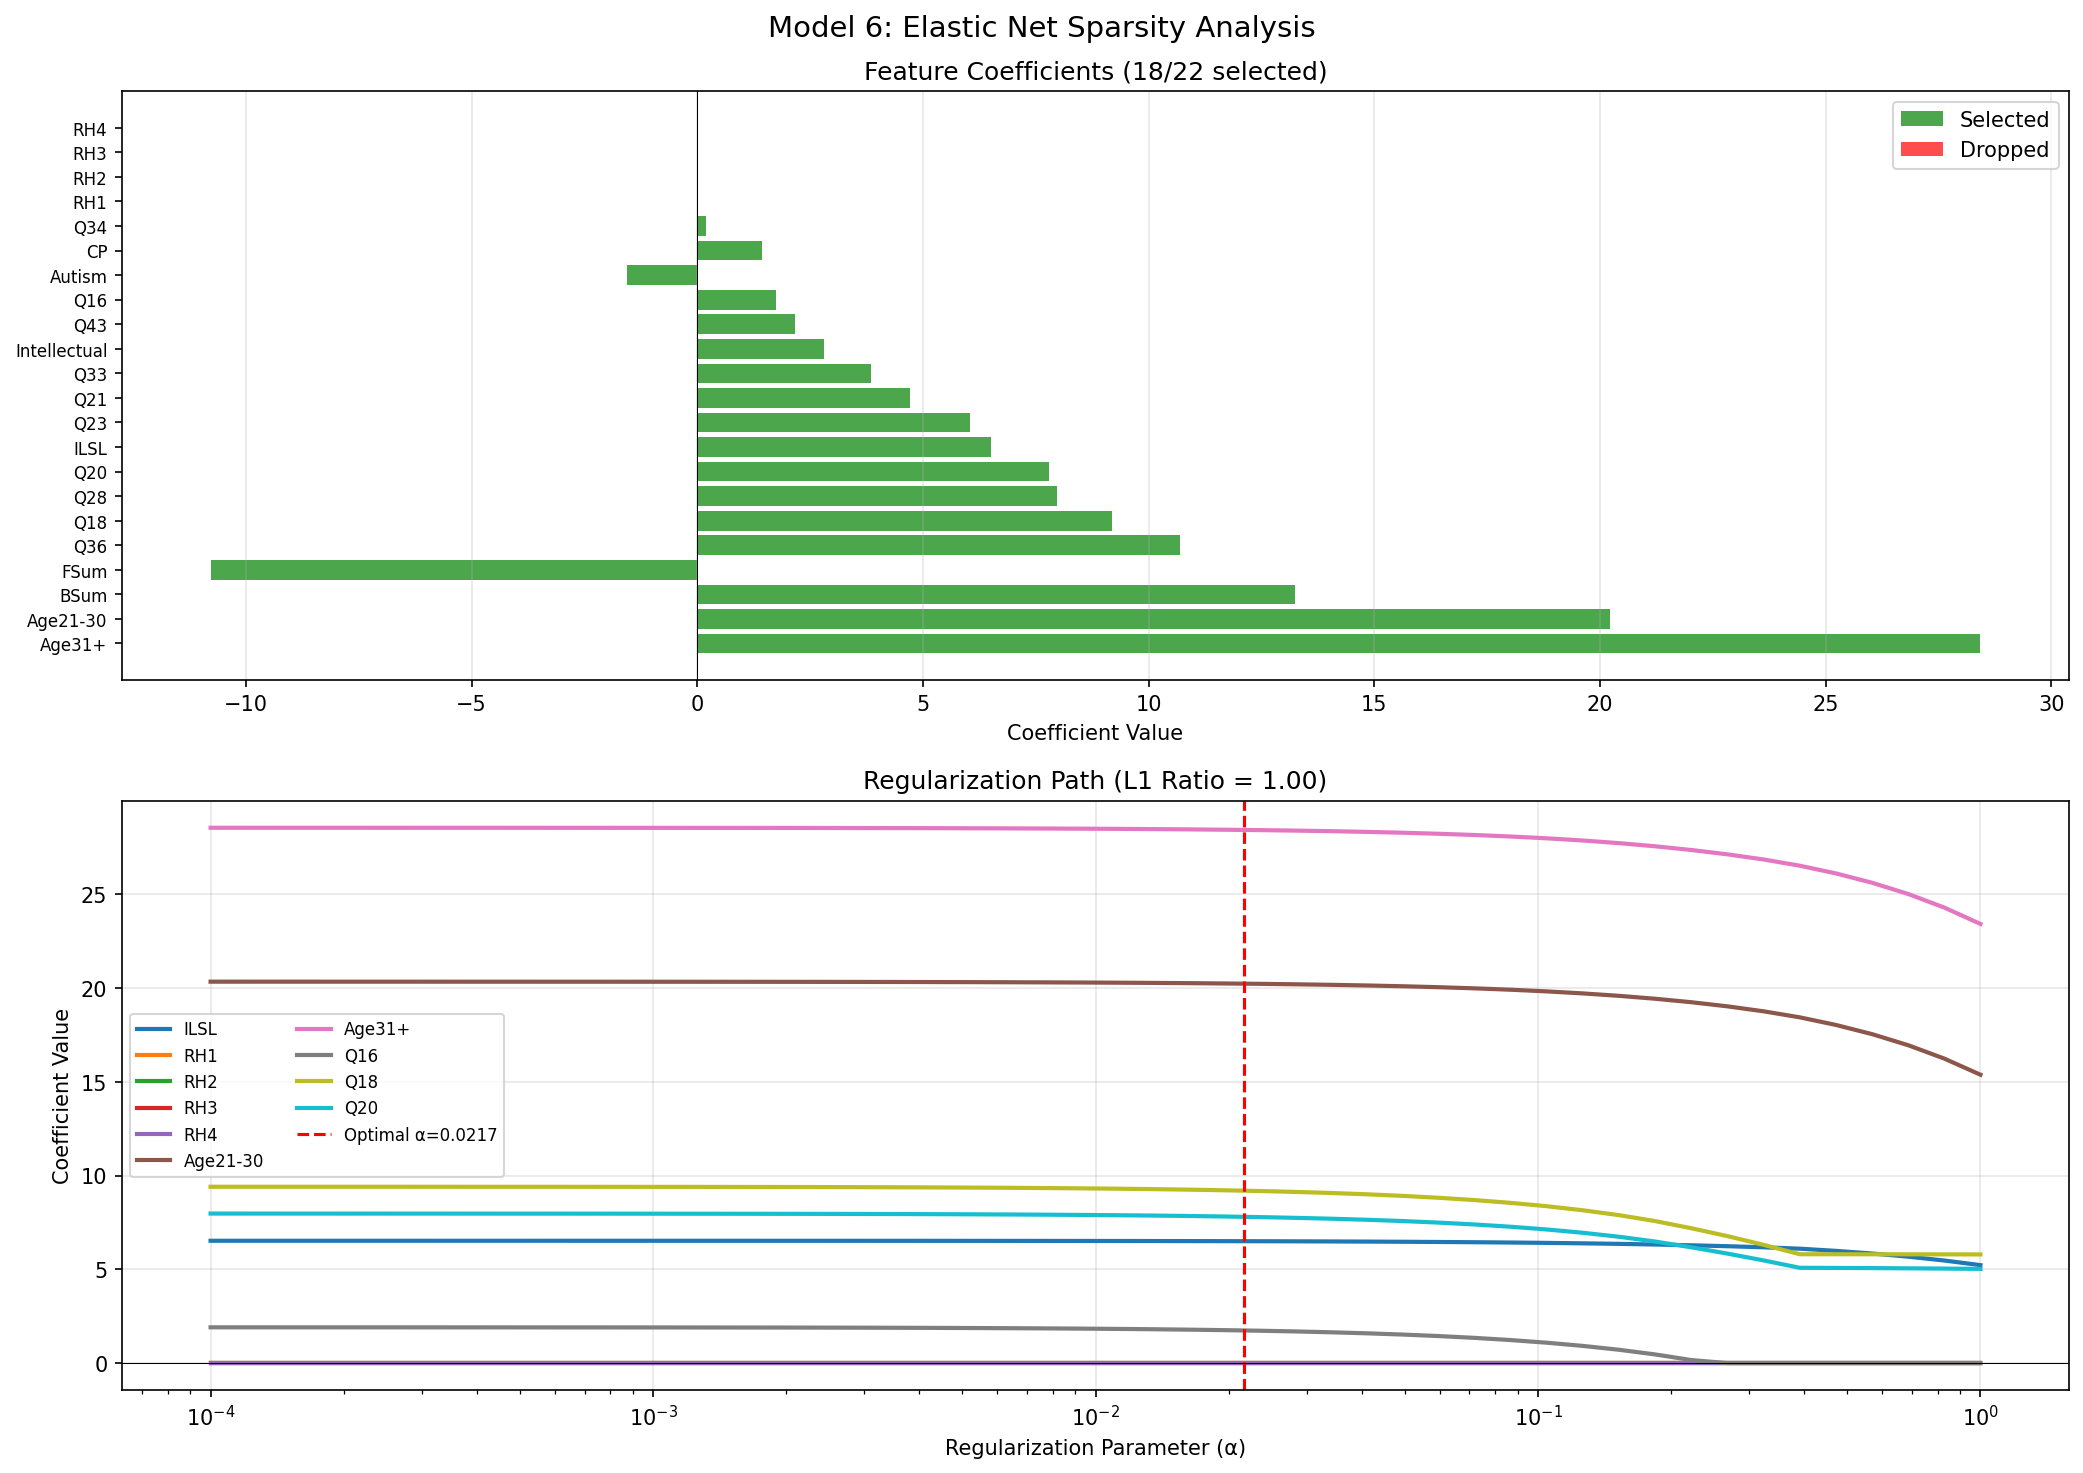
\includegraphics[width=\textwidth]{models/model_6/sparsity_analysis.png}
    \caption{Model 6 Sparsity Analysis and Regularization Path}
    \label{fig:model6_sparsity}
\end{figure}

\section{Comparison with Ridge Regression (Model 5)}

\begin{table}[h]
\centering
\caption{Elastic Net vs Ridge Comparison}
\begin{tabular}{lcc}
\toprule
\textbf{Characteristic} & \textbf{Ridge (Model 5)} & \textbf{Elastic Net (Model 6)} \\
\midrule
Features Used & All 22 & \ModelSixFeaturesSelected{} of 22 \\
Test R² & 0.7956 & \ModelSixRSquaredTest{} \\
Test RMSE & \$12,680 & \$\ModelSixRMSETest{} \\
Interpretability & Moderate & High \\
Feature Selection & None & Automatic \\
Coefficient Stability & High & High \\
Computational Cost & Low & Medium \\
\bottomrule
\end{tabular}
\end{table}

\section{Implementation Considerations}

\subsection{Advantages}

\begin{itemize}
    \item \textbf{Automatic Feature Selection}: Identifies the most predictive QSI questions and demographic factors
    \item \textbf{Reduced Complexity}: Simpler model with fewer active predictors
    \item \textbf{Enhanced Interpretability}: Clear identification of which factors drive costs
    \item \textbf{Stability}: L2 component prevents coefficient volatility
    \item \textbf{No Data Loss}: Uses 100\% of available data (no outlier removal)
\end{itemize}

\subsection{Challenges}

\begin{itemize}
    \item \textbf{Parameter Tuning}: Requires careful selection of $\alpha$ and L1 ratio
    \item \textbf{Feature Instability}: Selected features may vary with different data samples
    \item \textbf{Explanation Complexity}: Regularization concept may be difficult for stakeholders
    \item \textbf{Performance Trade-off}: Slight accuracy reduction compared to using all features
\end{itemize}

\section{Regulatory Compliance}

\begin{itemize}
    \item \textbf{F.A.C. 65G-4.0214}: Feature selection may complicate compliance if required questions are dropped
    \item \textbf{HB 1103 Transparency}: Feature selection enhances interpretability by identifying key drivers
    \item \textbf{Appeals Process}: Clearer with fewer active features
    \item \textbf{Documentation}: Selected features and coefficients must be clearly documented
\end{itemize}

\section{Recommendations}

\subsection{Primary Recommendation}

Elastic Net regression offers a valuable balance between prediction accuracy and model interpretability through automatic feature selection. The ability to identify which QSI questions and demographic factors are most predictive provides important insights for policy makers and can guide future data collection efforts.

\subsection{Implementation Strategy}

\begin{enumerate}
    \item \textbf{Validation Phase}: Test on historical data to verify feature selection stability
    \item \textbf{Stakeholder Communication}: Emphasize interpretability benefits
    \item \textbf{Documentation}: Maintain clear records of selected features and their coefficients
    \item \textbf{Regular Updates}: Re-tune parameters annually to adapt to changing patterns
    \item \textbf{Fallback Plan}: Maintain Ridge regression as backup if feature selection proves unstable
\end{enumerate}

\subsection{Risk Mitigation}

\begin{itemize}
    \item Monitor feature selection consistency across different data samples
    \item Validate that critical QSI questions are not inappropriately dropped
    \item Ensure regulatory compliance if certain features are mandated
    \item Provide clear explanations of the feature selection process
\end{itemize}

\section{Conclusion}

Model 6 (Elastic Net) successfully combines the benefits of automatic feature selection with prediction stability. With \ModelSixSparsityPercent{}\% of features retained and a test R² of \ModelSixRSquaredTest{}, the model achieves comparable performance to Ridge regression while providing enhanced interpretability through its identification of the most predictive factors.

The automatic selection of \ModelSixFeaturesSelected{} features from the original 22 simplifies the model and highlights which QSI questions and demographic factors are most important for predicting service costs. This insight can inform policy decisions and potentially streamline data collection processes.

While the regularization concept may require additional explanation for stakeholders, the interpretability benefits and maintained prediction accuracy make Elastic Net a strong candidate for implementation, particularly if understanding feature importance is a priority for the iBudget algorithm.